\documentclass[a4paper,10pt]{article}
\usepackage[utf8]{inputenc}
\usepackage{amsmath,amssymb}
\usepackage{enumerate}
\usepackage{ngerman}
\usepackage{graphicx}
\usepackage{ifpdf}
\usepackage[usenames]{color}
\usepackage[left=2.5cm,right=2.5cm,top=2.5cm,bottom=2.5cm]{geometry}
\usepackage[titles]{tocloft}
\usepackage[colorlinks=true,linkcolor=black]{hyperref}

\title{Pflichtenheft}
\date{}

\author{Usman Ghani Ahmed \\
Philip Caroli\\
Maximilian Madlung\\ 
Jeremias Mechler\\ 
Fabian Neundorf}

\ifpdf
\DeclareGraphicsExtensions{.pdf}
\else
\DeclareGraphicsExtensions{.eps}
\fi

% Einrückung bei Absätzen
\setlength{\parindent}{0mm}
% Zeilenabstand bei Absätzen
\setlength{\parskip}{2mm}

\begin{document}
 
\vspace{5cm}
\maketitle
\begin{center}
\vspace{3cm}
\huge{Praxis der Softwareentwicklung \\
Gruppe 3 \\[0.5cm]
Entwicklung eines "`Monopoly"'-ähnlichen Spiels \\[0.5cm]

\includegraphics[height=2cm]{kitlogo_de_rgb}  \\[0.5cm]
WS 2010 / 2011} \\[2cm]
%\textcolor{red}{! DRAFT !}
\end{center}
%damit machen
% 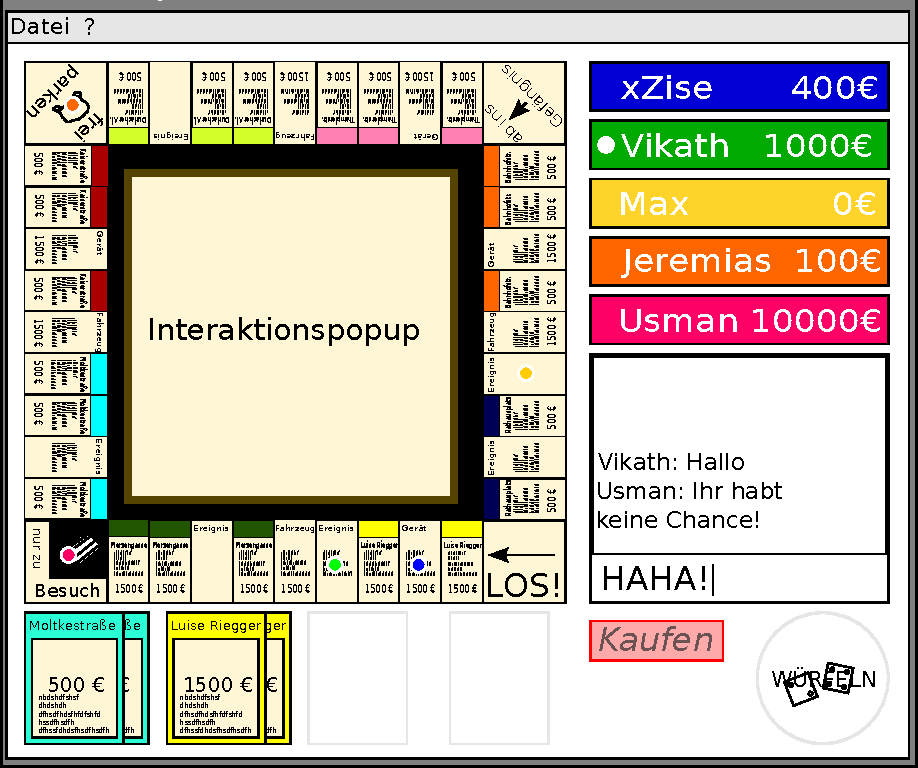
\includegraphics[height=15cm]{spielfeld}

\newpage

\tableofcontents

\newpage

\section{Produktübersicht}
Das Produkt ist eine Umsetzung des berühmten Brettspielklassikers "`Monopoly"' für den Computer.
Ziel des Spiels ist es, durch Geschicklichkeit, strategisches Denken und der nötigen Portion Glück das ganze Geld der Gegner einzunehmen. Gewonnen hat der Spieler, der zuletzt das meiste Geld besitzt. 

Das Spiel beinhaltet mehrere Spiel-Modi:
\begin{itemize}
\item Einzelspieler gegen Computer-KI
\item Mehrspieler an einem oder mehreren Computern sowie mit als auch ohne KI
\end{itemize}
Das Programm zeichnet sich durch seine Benutzerfreundlichkeit aus, die sich in der intuitiven Bedienbarkeit der graphischen Benutzeroberfläche äußert. Abgebildet werden das Monopoly\textregistered-Spielfeld sowie einige wenige zusätzliche Elemente, um die Übersichtlichkeit zu wahren. 
\subsection{Spielregeln}
Es können standardmäßig mindestens zwei und maximal acht Spieler an einem Spiel teilnehmen. Zu Beginn des Spieles bekommt jeder Spieler ein festgelegtes Startkapital, mit dem er Straßen, Häuser und Hotels kaufen kann oder Strafen sowie Steuerzahlungen die durch Ereignisse entstehen an die Bank bzw. in die Mitte des Spielbretts bezahlen muss. 

Auf einer Straße kann man zusätzlich noch Hotels und Häuser bauen, dadurch erhöht sich die Miete der Straße. Das Geld, das sich auf dem Spielbrett sammelt, bekommt derjenige Spieler, der auf dem Feld ``Frei parken'' zum Stehen kommt.  Es treten verschiedene Spieler gegeneinander an, dabei können die Spieler menschlich sein oder werden vom Computer (KI) gesteuert.

Jeder Spieler kommt abwechselnd und zyklisch an die Reihe und würfelt mit zwei Würfel. Die Summe, die sich aus den Augenzahlen der zwei Würfel ergibt, gibt dem Spieler Auskunft darüber, wie viele Schritte er mit seiner symbolischen Figur voranschreiten darf. Die Spielfiguren bewegen sich im Uhrzeigersinn auf dem Spielfeld. Dabei überquert der Spieler im Laufe des Spiels verschiedene Straßen, die von Spielern für einen festgelegten Preis gekauft werden können. Bleibt der Spieler auf einer Straße, die einem anderen Spieler gehört, stehen, so muss er einen gewissen Betrag an Geld an diesen Spieler zahlen (Miete). Die Höhe des Einnahmegeldes (Miete) hängt davon ab, ob der Spieler nur diese Straße besitzt oder ob er auf dieser Straße noch weitere Gebäude (Häuser, Hotels) gebaut bzw. gekauft hat. Wenn der Spieler zusätzlich noch Häuser und Hotels auf dieser Straße gebaut hat, dann erhöht sich das Einnahmegeld für die jeweilige Straße. Dabei steigt die Miete in aufsteigender Reihenfolge, d.h die Miete für ein Hotel ist höher als die für ein Haus.
	
Landet der Spieler auf einem ``Steuern bezahlen''-Feld,dann muss er Steuern bezahlen, die sich in der Mitte des Spielbretts sammeln. Bleibt der Spieler auf dem  Feld "`Gefängnis"' stehen, so setzt er eine Würfelrunde aus, kann jedoch immer noch Miete von den anderen Spielern einnehmen, sowie Handel mit anderen Spielern betreiben. Überquert ein Spieler  das Feld "`Los"', auf welchem zu Beginn gestartet wurde, so kassiert er eine Prämie. Beim Stillstand auf einem Ereignisfeld zieht der Spieler eine Ereigniskarte mit verschiedenen Aufgaben, die der Spieler erledigen muss und dabei auch Geldprämien kassieren kann oder Abgaben bezahlen muss.  Jeder Spieler hat während des Spiels die Möglichkeit, seine Gebäude und Straßen an die anderen Spieler zu verkaufen, sowie diese für eine Ersteigerung (Auktion) freizugeben. Kann ein Spieler finanziell seinen Forderungen nicht mehr nachkommen, so scheidet er automatisch aus. Spieler, die vorzeitig ein laufendes Spiel beenden, können ihre Habe entweder an die Bank abgeben oder an ihre Mitspieler. Gewonnen hat der Spieler, der zuletzt das meiste Geld besitzt. Ziel dieses Spieles ist, durch Geschicklichkeit und ein bisschen Glück seine Gegner finanziell in die Knie zu zwingen.
\newpage
\section{Zielbestimmung}
\subsection{Musskriterien}
\begin{itemize}
\item Plattformunabhängigkeit (Java, Swing)
\item Umsetzung der Monopoly-Regeln
\item Client-Server-Architektur
\item Spielen gegen KI-Client mit Fähigkeitslevel eines Monopoly-Anfängers möglich
\item Anzeigen und Interaktion mit dem Spielfeld in Form einer grafischen Benutzeroberfläche
\item Spielen mit variabler Anzahl echter Spieler und KI-Spieler auf einem Server gegeneinander möglich
\end{itemize}
\subsection{Sollkriterien}
\begin{itemize}
\item Spielplan, Text und Grafik sind variabel
\item Benutzeroberfläche sieht dem Monopoly-Brett ähnlich
\item Netzwerkfähigkeit
\end{itemize}
\subsection{Kannkriterien}
\begin{itemize}
\item Spielregeln lassen sich variieren
\item Lokalisierbarkeit
\item Text-Chat
\item Zuschauermodus
\item Server-Admin kann Spiel verwalten
\item Unterbrechen, Speichern und Fortsetzen eines Spiels
\item Hilfe
\end{itemize}
\subsection{Abgrenzungskriterien}
\begin{itemize}
\item Umsetzung für mobile Systeme 
\item Finden von Internetservern (Metaserver)
\item Voice-Chat
\item verschiedene KI-Stufen
\end{itemize}
\newpage
\section{Produkteinsatz}
\subsection{Anwendungsbereiche}
\begin{itemize}
\item Privater PC, Freizeit
\end{itemize}
\subsection{Zielgruppen}
\begin{itemize}
\item Menschen mit Spaß an Gesellschaftsspielen aus dem deutschsprachigen Raum
\end{itemize}
\subsection{Betriebsbedingungen}
\begin{itemize}
\item Dauer eines Spiels: Circa ein bis drei Stunden
\end{itemize}
\section{Produktumgebung}
\subsection{Software}
\begin{itemize}
\item Java Runtime Environment SE 1.6 oder neuer
\item Betriebssystem zum Beispiel Windows, Linux, OS X
\end{itemize}
\subsection{Hardware}
Mindestanforderungen (PC): 
\begin{itemize}
\item 128 MB Arbeitsspeicher
\item 100 MB freien Festplattenspeicher
\item 500-MHz-Prozessor
\item Bildschirmauflösung: 1024 $\times$ 768
\item Beschleunigte 2D-Grafik
\end{itemize}
Empfohlen:
\begin{itemize}
\item 512 MB Arbeitsspeicher
\item 100 MB freien Festplattenspeicher
\item 1-GHz-Prozessor
\item Bildschirmauflösung: 1280 $\times$ 1024
\item Beschleunigte 2D-Grafik
\item Netzwerk- oder Internetverbindung (TCP/IP, IPv4)
\end{itemize}
\subsection{Orgware}
entfällt
\subsection{Schnittstellen}
\begin{itemize}
\item Vorgegebene Client-Server-Schnittstelle (Java-Interface)
\item Netzwerk-Client-Server-Schnittstelle
\end{itemize}
\section{Funktionale Anforderungen}
Jede funktionale Anforderung wird durch eine fünfstellige Nummer gekennzeichnet. Die erste Stelle gibt die Anwendung an:
\begin{enumerate}
\item Client
\item Server
\item KI-Client
\end{enumerate}
Die zweite Stelle gibt den Bereich innerhalb des Spielverlaufs an.
\begin{enumerate}
\item Vorbereitungen
\item Spielzug
\end{enumerate}
Die drei letzen Stellen werden dann durchnummeriert.
\subsection{Client}
\subsubsection{Außerhalb des Spielfeldes}
\begin{description}
\item[/F11010/] Anzeigen des Hauptmenüs \\
Beim Starten des Programms soll das das Hauptmenü angezeigt werden.

Im Hauptmenü können folgende Punkt angewählt:
\begin{itemize}
\item Einstellungen ($\rightarrow$ /F11020/)
\item Spiel erstellen ($\rightarrow$ /F11050/)
\item Spiel beitreten ($\rightarrow$ /F11100/)
\item Spiel speichern ($\rightarrow$ /F11700/) (nur bei aktivem Spiel)
\item Beenden
\end{itemize}

\item[/F11020/] Ändern der Spieleinstellungen \\
Zuerst werden die Einstellungen geladen und in das Fenster übertragen ($\rightarrow$ /F11030/). Danach kann man diese ändern und können dann gespeichert werden ($\rightarrow$ /F11040/).

\item[/F11030/] Laden der Einstellungen \\
Die in den Einstellungen ($\rightarrow$ /F11020/) vorhandenen Daten werden vor dem Anzeigen aus der Datei geladen.

\item[/F11040/] Speichern der Einstellungen \\
Die im Einstellungsfenster ($\rightarrow$ /F11020/) eingestellten Einstellungen werden gespeichert.

\item[/F11050/] Erstellen eines Servers (Konfiguration) \\
Es ist möglich einen Server zu starten. Dazu kann man eine Konfiguration laden ($\rightarrow$ /F11060/), ändern und speichern ($\rightarrow$ /F11070/). Alternativ kann auch ein Spielstand geladen werden ($\rightarrow$ /F11160/). Danach kann der Server dann gestartet werden.

\item[/F11060/] Laden der Einstellungen \\
Die im Konfigurationsfenster des Servers ($\rightarrow$ /F11050/) angezeigten Einstellungen werden vor dem Anzeigen aus der Datei ($\rightarrow$ /DB02/) geladen.

\item[/F11070/] Speichern der Einstellungen \\
Die in den Einstellungsfenster ($\rightarrow$ /F11050/) eingestellten Einstellungen werden gespeichert.

\item[/F11080/] Erstellen eines Servers \\
Nachdem die Einstellungen durchgeführt wurden ($\rightarrow$ /F11050/) kann ein Server gestartet werden, dadurch wird ($\rightarrow$ /F11090/) aufgerufen.

\item[/F11090/] Starten eines Servers \\
Ein Server wird initialisiert und gestartet, er befindet sich dann im Bereitschaftsmodus und stellt den Spielern einen "`Warteraum"' zur Verfügung.

\item[/F11100/] Spiel beitreten \\
Im Hauptmenü ($\rightarrow$ /F11010/) kann einem Spiel beigetreten werden, je nach Benutzerwahl können dann "`Direkte Verbindung"'($\rightarrow$ /F11110/) oder die "`Serverliste"' ($\rightarrow$ /F11120/) ausgewählt werden. Danach wird ein eventuell vorhandenes Passwort und die Namen sowie die Anzahl der Spieler abgefragt und dann die Verbindung aufgebaut ($\rightarrow$ /F12010/). Sofern das Spiel bereits läuft wird, der Vorgang abgebrochen.

\item[/F11110/] Spiel beitreten durch Eingabe einer IP (direkte Verbindung) \\
Die IP wird angenommen und es wird getestet, ob mit der IP ein Server erreichbar ist und Plätze frei hat. Sind keine Plätze frei, wird damit abgebrochen.

\item[/F11120/] Anzeigen der Serverliste \\
In dieser Liste können einige Server angezeigt werden, ohne dessen IP zu kennen ($\rightarrow$ /F11130/).

In dieser Liste kann ein Server angewählt werden, sofern noch Plätze frei sind. Ansonsten ist eine Verbindung nicht möglich.
\item[/F11130/] Ermitteln der Server im lokalen Netzwerk \\
Die im Netzwerk verfügbaren Server werden auf die Liste aufgenommen und die Serverinformationen werden abgefragt.

\item[/F11140/] Abfragen der Serverinformationen für die Serverliste \\
Jeder Server in der Liste übersendet wichtige Informationen über sich, um sie dann in der Liste anzuzeigen (z.\,B. ob ein Passwort vorhanden ist, wie viele Spieler sich verbunden haben, wie viele Spieler sich verbinden dürfen).

\item[/F11150/] Verlassen des Spiels \\
Über die entsprechende Schaltfläche im Programm kann das Spiel verlassen werden.

\item[/F11160/] Spielstand laden \\
Sofern man ein Spielstand lädt wird die Konfiguration automatisch daraus geladen.

\item[/F11170/] Spielstand speichern \\
Man kann im Hauptmenü den Spielstand jederzeit speichern.
\end{description}

\subsubsection{Bei hergestellter Verbindung}
\begin{description}
\item[/F12010/] Initiieren eines Spiels \\
Der Warteraum wird angezeigt. Währenddessen kann man sich mit den anderen Spielern unterhalten ($\rightarrow$ /F12020/). Nachdem mindestens zwei Spieler verbunden sind und alle Spieler bereit sind, startet das Spiel ($\rightarrow$ /F12030/). 
\item[/F12020/] Chatten \\
Es ist während des gesamten Spiels möglich, mit anderen Spielern zu chatten.

\item[/F12030/] Starten des Spiels \\
Nachdem das Spiel gestartet ist, erscheint bei allen das Spielfeld, auf dem folgende Punkte angezeigt werden:
\begin{itemize}
\item Spieler mit deren Namen und Kontostände
\item Die Straßen mit deren Zugehörigkeit und Bebauung
\item Die Spielfiguren
\item Interaktionspopup
\begin{itemize}
\item Das Geld in der Mitte
\item Handel
\item Versteigerungen
\item Ereigniskarten
\end{itemize}
\item Das Chatfenster
\end{itemize}
Daraufhin kann er der erste Spieler die Runde starten ($\rightarrow$ /F12040/). Außerdem kann jeder während des gesamten Spiels Nachrichten versenden ($\rightarrow$ /F12020/).
\item[/F12040/] Durchführung einer Runde \\
Sobald der nächste Spieler aktiv ist, darf dieser selber würfeln und somit den Zug beginnen ($\rightarrow$ /F12050/).
\item[/F12050/] Würfeln \\
Zum Würfeln fragt der aktive Spieler eine Zufallszahl beim Server ab ($\rightarrow$ /F22020/). Anhand dieser Zufallszahl ziehen die Spieler die Spielfigur des aktiven Spielers weiter.

Landet der Spieler auf einen Sonderfeld, wird entsprechend dem Sonderfeld vorgegangen. Danach kann der aktive Spieler weitere Aktionen durchführen ($\rightarrow$ /F12060/).
\item[/F12060/] Weitere Aktionen \\
Nachdem der Spieler gewürfelt hat, kann er folgende Aktionen ausführen:
\begin{itemize}
\item den Spielzug beenden ($\rightarrow$ /F22010/ /F12040/).
\item eine Straße kaufen ($\rightarrow$ /F22031/ /F12061/).
\item ein Gebäude bauen ($\rightarrow$ /F22032/ /F12062/).
\item eine Hypothek aufnehmen ($\rightarrow$ /F22033/ /F12063/).
\item ein Gebäude abreißen ($\rightarrow$ /F22034/ /F12064/).
\item einen Handel initiieren ($\rightarrow$ /F22035/ /F12065/).
\item eine Straße versteigern ($\rightarrow$ /F22036/ /F12066/).
\end{itemize}
Außerdem kann währenddessen die Miete vom Besitzer der Straße eingefordert werden ($\rightarrow$ /F12070/).
\item[/F12061/] Straße kaufen \\
Da der Spieler nur die Straße kaufen kann, auf den der Spieler steht, wird vorher nur geprüft, ob die Straße zu verkaufen ist und der Spieler genügend Geld hat ($\rightarrow$ /F22031/). Danach kann der Spieler weitere Befehle ausführen ($\rightarrow$ /F120Y0/).
\item[/F12062/] Gebäude bauen \\
%alternativ: Der Spieler fragt einfach den Server
Zuerst wird geprüft, ob der Spieler genügend Geld hat und nach den entsprechenden Regeln dort ein Gebäude gebaut werden darf. ($\rightarrow$ /F22032/)
\item[/F12063/] Hypothek aufnehmen \\
Wenn der Spieler nach den Regeln eine Hypothek aufnehmen darf, meldet der aktive Spieler dies dem Server ($\rightarrow$ /F22033/).
\item[/F12064/] Gebäude abreißen \\
Erst wird überprüft, ob der Spieler das Gebäude nach den Spielregeln abreißen darf ($\rightarrow$ /F22034/).
\item[/F12065/] Handel initiieren \\
Der aktive Spieler kann ein Handel mit einem anderen Spieler oder der Bank initiieren ($\rightarrow$ /F22035/). Darauf hin können beide Spieler ihr Angebot einstellen und dieses fixieren. Danach müssen beide dann das Angebot bestätigen und der Handel erfolgt.
\item[/F12066/] Straße versteigern \\
Um eine Straße zu versteigern, müssen dies die Regeln erlauben. Danach kann jeder Spieler darauf bieten ($\rightarrow$ /F22036/).
\item[/F12070/] Miete erheben \\
Sobald ein Spieler auf ein Feld zieht, das ihm nicht gehört, kann der Besitzer die Miete erheben. Dies kann er solange, bis der nächste Spieler gewürfelt hat.

Nachdem der Spieler fertig ist, kann er die aktuelle Runde an den nächsten Spieler abgeben. Außerdem kann ein Spieler aufgeben ($\rightarrow$ /F20/).
\item[/F12080/] Aufgeben \\
Jeder Spieler kann, sobald er an der Reihe ist, aufgeben. Er kann dann sagen, was mit seinem verbleibenden Besitz passiert:
\begin{itemize}
\item Die Bank bekommt das Geld, die Ereigniskarten und die Straßen zurück. Je nach Einstellungen bleiben die Gebäude stehen oder werden abgerissen.
\item Zuerst werden alle Straßen an andere Spieler versteigert, dann bekommt die Bank die übrig gebliebenen Straßen, das Geld und die Ereigniskarten. Wieder können je nach Einstellungen die Gebäude stehen bleiben.
\item Es ist möglich, das Eigentum an andere Spieler zu verschenken. Alles Übriggebliebene geht an die Bank. Eventuell vorhandene Straßen mit Gebäuden behalten die Gebäude abhängig von den Einstellungen.
\end{itemize}
\end{description}

\subsection{Server}
\subsubsection{Vorbereitungen}
\begin{description}
\item[/F21010/] Starten des Servers \\
Bei den Starten des Servers wird ermittelt, ob ein Spielstand geladen ($\rightarrow$ /F21020/) oder ein neues Spiel gestartet werden soll ($\rightarrow$ /F21030/).
\item[/F21020/] Spielstand laden \\
Sofern der Spielstand valide ist, wird diese Datei eingelesen und der Server ist im Wartemodus ($\rightarrow$ /F21040/).
\item[/F21030/] Neues Spiel starten \\
Es wird ein neues Spiel gestartet, indem die entsprechenden Anfangseinstellungen aus den Übergabeparametern oder einer Datei geladen werden. Danach befindet sich der Server im Wartemodus ($\rightarrow$ /F21040/).
\item[/F21040/] Wartemodus \\
Im Wartemodus stellt der Server einen Chatraum zur Verfügung. Jeder Spieler landet zuerst hier und kann sich auf `bereit"' setzen. Nachdem mindestens zwei Spieler verbunden und alle bereit sind, startet das Spiel ($\rightarrow$ /F21050/), sofern es sich um ein geladenes Spiel handelt. Ansonsten, wenn es sich um ein neues Spiel handelt, werden die Vorbereitungen abgeschlossen ($\rightarrow$ /F21060).
\item[/F21050/] Spielstart \\
Nachdem allen Spieler die Reihenfolge übermittelt wurde, wird der erste Spielzug gestartet, indem der entsprechende Spieler informiert wird, dass er dran ist ($\rightarrow$ /F22040/).
\item[/F21060/] Vorbereitungen eines neuen Spiels abschließen \\
Wenn es sich um ein neues Spiel handelt, wird die Reihenfolge der Spieler festgelegt, und der erste Spieler in der neuen Reihenfolge ist dann der erste Spieler der einen Zug ausführen darf. Danach startet das Spiel ($\rightarrow$ /F21050).
\end{description}
\newpage
\subsubsection{Spielzug}
\begin{description}
\item[/F22010/] Spielzug informieren \\
Nachdem die Person bekannt ist, die nun zieht, wird allen Spielern übermittelt, dass dieser Spieler dran ist. Danach wartet der Server darauf, dass gewürfelt werden soll ($\rightarrow$ /F22020/). Währenddessen stellt der Server einen Chatraum zur Verfügung. Überschreitet der aktive Spieler eine Bedenkdauer, wird der Spieler herausgeworfen und alles geht an die Bank.
\item[/F22020/] Würfeln \\
Um den Betrug des Spielers vorzubeugen, bekommt der Server von den Client den Befehl zu würfeln. Dieser erzeugt dann eine zufällige Zahl zwischen 2 und 12. Alle Spieler erhalten dann diese Zahl und alle Spieler ziehen die Spielfigur des aktiven Spielers weiter. Danach kann der aktive Spieler weitere Befehle geben ($\rightarrow$ /F22030/).
\item[/F22030/] Weitere Befehle \\
Der Server bekommt jetzt die weiteren Befehle vom entsprechenden Client. Bei allen der folgenden Befehle wird anfangs getestet ob der Zug erlaubt ist:
\begin{itemize}
\item Der nächste Spieler kann an der Reihe sein ($\rightarrow$ /F22010/).
\item Der Spieler möchte die Straße kaufen ($\rightarrow$ /F22031/).
\item Der Spieler möchte ein Gebäude bauen ($\rightarrow$ /F22032/).
\item Der Spieler kann eine Hypothek aufnehmen ($\rightarrow$ /F22033/).
\item Der Spieler kann ein Gebäude abreißen ($\rightarrow$ /F22034/).
\item Der Spieler kann handeln ($\rightarrow$ /F22035/).
\item Der Spieler kann eine Straße versteigern ($\rightarrow$ /F22036/).
\item Der Spieler kann aussteigen ($\rightarrow$ /F22037/).
\end{itemize}
Alle Spieler werden darüber nach erfolgreicher Ausführung informiert.
\item[/F22031/] Kauf einer Straße \\
Der Kontostand des Spielers wird entsprechend des Kaufpreises belastet und als Besitzer der Straße der aktuelle Spieler eingetragen.
\item[/F22032/] Bau eines Gebäudes \\
Der Kontostand wird mit den Gebäudepreis belastet und der Straße ein Gebäude hinzugefügt.
\item[/F22033/] Aufnehmen einer Hypothek \\
Bei der Aufnahme der Hypothek wird der Kontostand des Spielers erhöht.
\item[/F22034/] Gebäudeabriss \\
Dem Kontostand wird der entsprechende Abrisswert hinzugefügt und das Gebäude von der Straße entfernt.
\item[/F22035/] Handel \\
Beim Handel wird der Handelspartner über den Beginn eines Handels informiert. Dann können beide Spieler ihre Angebote hinzufügen ($\rightarrow$ /F22041/). Sofern ein Spieler fertig ist, kann dieser das Angebot fixieren und keine Änderungen an dem eigenen Angebot vornehmen. Sobald beide das als Angebot fixiert haben, können diese es annehmen und der Handel erfolgt.
\item[/F22036/] Versteigern einer Straße \\
Zuerst wird getestet, ob die Spielregeln es erlauben, die Straße zu verkaufen. Sofern die Regeln es erlauben, wird die Straße den Personen zum Verkauf angeboten. Alle Spieler können dann darauf bieten und entsprechend den Preis erhöhen. Nach der Versteigerung werden alle Spieler über den neuen Besitzer der Straße informiert.
\item[/F22037/] Ausstieg eines Spielers \\
Ein Spieler kann aussteigen und seinen Besitz entweder an die Bank zurückgeben, verkaufen oder versteigern.
\item[/F22040/] Spielstand speichern \\
Es gibt einen Befehl um den Spielstand zu speichern.
\end{description}

\subsection{KI Client}
\subsubsection{Vorbereitungen}
\begin{description}
\item[/F31001/]Starten des KI-Client\\
Der KI-Client verbindet sich beim Start automatisch mit einem Server, dessen Beschreibung er per Befehlsparameter erhalten muss
\item[/F31002/]Betreten eines Servers\\
Wenn der KI-Client einem Server beitritt, setzt er sich automatisch auf "`bereit"' und wartet auf den Beginn des Spiels
\item[/F31003/] Laden der KI-Parameter \\
Der Client lädt die Parameter für seine KI-Logik aus einer angegebenen Datei
\end{description}
\subsubsection{Spielzug}
\begin{description}
\item[/F32001/] Durchführen eines Zuges\\
Der KI-Client würfelt automatisch und kann danach alle Spielaktionen ausführen, die auch der Spielerclient ausführen kann.
\item[/F32002/] Ausführen einer Spielaktion \\
Die interne KI-Spiellogik entscheidet, ob und welche Aktion ausgeführt werden soll
\item[/F32030/] Verlangen der Miete \\
Sobald ein anderer Spieler auf einem Spielfeld, das dem KI-Klienten gehört landet, verlangt dieser die anfallende Miete
\item[/F32004/]Speichern der KI-Parameter \\
Sobald sich die KI-Parameter verändern, werden die neuen Parameter in der Datei gespeichert, aus der sie in /F31003/ geladen wurden
\end{description}

\section{Produktdaten}
\subsection{Allgemein}
Folgende Daten müssen sowohl Server als auch Client vorliegen:
\begin{description}
\item[/PD01/] Spielfeld
\begin{itemize}
\item Straßennamen
\item Währungszeichen, Währungsnamen
\item Beschriftung der Sonderfelder (``Frei parken'' usw)
\item Text der Ereigniskarten
\item Name / Beschreibung der baubaren Objekte
\item optional: Grafiken für die Spielfelder
\end{itemize}
\end{description}

\subsection{Server}
\begin{description}
\item[/PD02/] Servereinstellungen
\begin{itemize}
\item Servername
\item Passwort (optional)
\item Mindestspielerzahl
\item Höchstspieleranzahl
\end{itemize}
\item[/PD03/] Spielstand
\begin{itemize}
\item Liste aller teilnehmenden Spieler
\item Kontostand jedes Spielers
\item Besitz an Spielfeldern und Gebäuden jedes Spielers
\item Hypotheken auf Spielfeldern
\item aktueller Spieler
\item Verteilung der Ereigniskarten
\item Anzahl und Name der KI-Clients
\end{itemize}
\end{description}

\subsection{Client}
\begin{description}
\item[/PD04/] Client-Einstellungen
\begin{itemize}
\item Spielername
\item IP des zuletzt beigetretenen Servers
\item präferenzierte Größe des Fensters
\end{itemize}
\end{description}

\subsection{KI-Client}
\begin{description}
\item[/PD05/] KI-Einstellungen
\begin{itemize}
\item Name (optional)
\item Parameter der KI-Logik
\end{itemize}
\end{description}

\section{Produktleistungen}
Zeit:
\begin{itemize}
\item Starten eines Servers: $<$ 15 Sekunden
\item Beitreten eines Servers: $<$ 15 Sekunden
\item Öffnen des Hauptmenüs: $<$ 15 Sekunden
\item Ausführen einer Aktion: $<$ 2 Sekunden
\item Erkennen eines Verbindungsabbruchs: $<$ 30 Sekunden
\item Beenden eines Spiels: $<$ 10 Sekunden
\end{itemize}
Genauigkeit:
\begin{itemize}
\item Alle Aktionen sollen genau / fehlerfrei zwischen Server und Client übertragen werden
\end{itemize}
\newpage
\section{Weitere nichtfunktionale Anforderungen}
Urheber- und Markenrechte:
\begin{itemize}
\item "`Monopoly"' ist ein eingetragenes Warenzeichen, d.h. das Produkt darf nicht "`Monopoly"' oder einen ähnlich klingenden / verwechselbaren Namen tragen
\item Der Spielplan, das Regelwerk (als Textstück), die Figuren und alle Graphiken sind unter Schutzrecht, d.h. die sichtbaren Elemente des Produkts müssen von diesen Abweichen
\item Spielregeln sind generell nicht schutzfähig (Patentgesetz und Gebrauchsmustergesetz 1.2), wobei der genaue Regelaufbau vielleicht trotzdem noch verändert werden sollte.
\end{itemize}
Sicherheitsanforderungen:
\begin{itemize}
\item Es darf nicht möglich sein, durch Server oder Client des Produktes andere Programme o.ä. zu beeinflussen
\item Alle Spielaktionen sollten vom Server verifiziert werden, um "`Cheaten"' zu verhindern
\end{itemize}
Plattformabhängigkeiten:
\begin{itemize}
\item Das Produkt muss auf der offiziellen Java-VM von Oracle laufen
\end{itemize}
\section{Qualitätsanforderungen}
\begin{itemize}
\item Das Produkt muss zuverlässig laufen und darf nicht ohne ausführliche Fehlermeldung crashen
\item Es müssen durchschnittlich mindestens fünf Spiele in Folge gespielt werden können, ohne dass ein Fehler auftritt
\item Das Programm verhält sich Verbindungsabbrüche betreffend robust und versucht bei Auftreten eines solchen das Spiel wiederherzustellen 
\item Es muss möglich sein, nach einem Fehler einem angefangen Spiel wieder beizutreten (Client) bzw. ein Spiel wieder so zu Starten wie es vor dem Fehler lief (Server)
\end{itemize}
\newpage
\section{Globale Testfälle und Testszenarien}
Folgende Funktionssequenzen sind in der grafischen Benutzeroberfläche durchzuführen. Der Server wird entsprechend mitgeprüft: \\
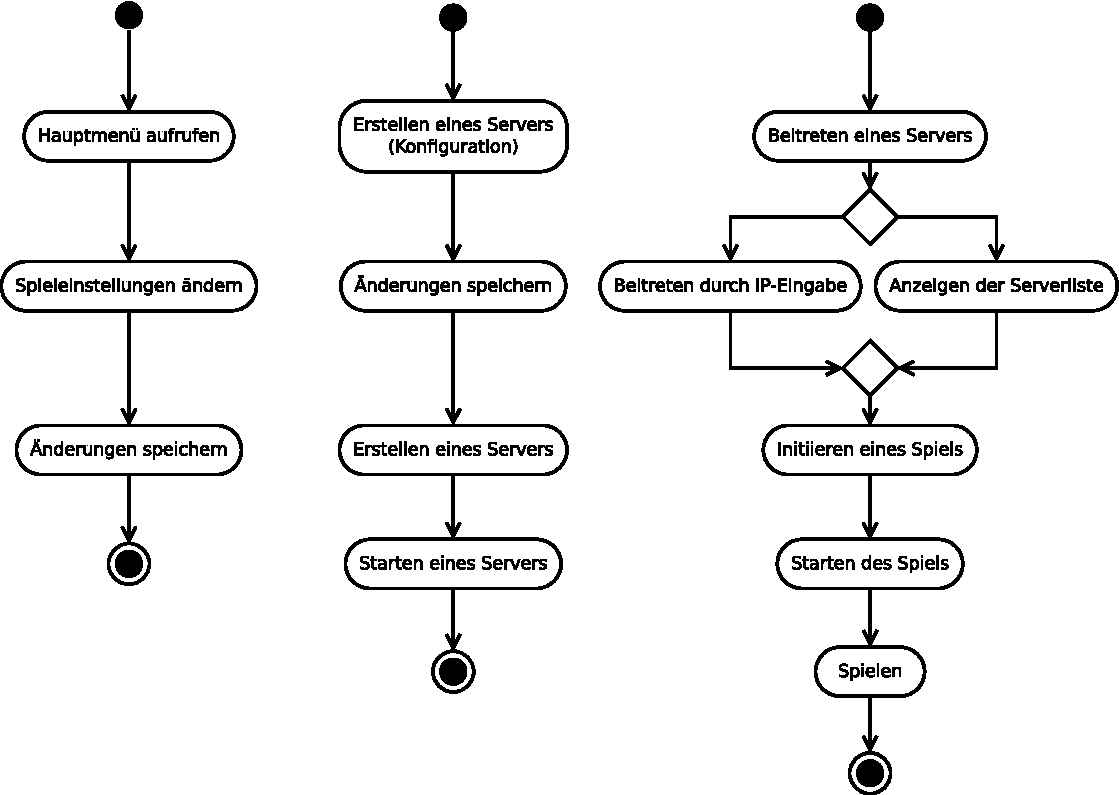
\includegraphics[width=17cm]{Diagram1} \\
Folgende Datenkonsistenzen müssen eingehalten werden:
\begin{itemize}
\item Zu jedem Zeitpunkt muss ein Spielername definiert sein
\item Einstellungen können nur geladen werden, wenn die zu ladende Datei vollständig ist
\item Einstellungen können nur gespeichert werden, wenn alle Felder korrekt ausgefüllt sind
\item Der Zustand des Spielfeldes muss zwischen Client und Server identisch sein
\end{itemize}
Folgende unzulässigen Aktionen müssen korrent behandelt werden:
\begin{itemize}
\item Unzulässiges Übersenden von Kommandos an Client und Server (DoS)
\item Überschreitung der maximalen Teilnehmeranzahl
\item Belegung von Ressourcen durch häufiges Beitreten und Verlassen von Clients
\item Unerwarteter Verbindungsabbruch (Timeout, Connection Reset)
\item Reaktion auf Verbindungsverlust zum Server
\item Unsauberer Restart des Clients
\item Übersenden von undefinierten und unzulässigen Befehlen an Client und Server
\end{itemize}
\newpage
Interoperabilität, Usability:
\begin{itemize}
\item Richtige Funktion mit Client und Server der anderen Gruppe
\item Korrekte Darstellung auf verschiedenen Betriebssystemen (Windows, Linux, OS X)
\item Verschiedene Bildschirmauflösungen
\item nicht-standardmäßige Systemschriftgröße
\end{itemize}
Testszenarien:
\begin{itemize}
\item ``Erste Inbetriebnahme mit Starten eines Servers'' \\
Starten des Programms $\rightarrow$ im Hauptmenü "`Einstellungen"' aufrufen $\rightarrow$ Daten eingeben $\rightarrow$ ``Spieleinstellungen speichern'' anklicken $\rightarrow$ im Hauptmenü ``Spiel erstellen'' anklicken $\rightarrow$ Einstellungen vornehmen $\rightarrow$ ``Einstellungen speichern'' anklicken $\rightarrow$ ``Erstellen des Servers'' anklicken $\rightarrow$ ``Starten des Servers'' anklicken.
\item ``Einem Spiel beitreten (durch Serverliste), spielen und aufgeben'' \\
Starten des Programms $\rightarrow$ ``Spiel beitreten'' auswählen$\rightarrow$ "`Serverliste"' anklicken $\rightarrow$ Server auswählen $\rightarrow$ verbinden $\rightarrow$ Bereitschaft setzen $\rightarrow$ Würfeln, Spielzüge durchführen $\rightarrow$ aufgeben
\item "`Einzelspieler"' \\
``Spiel erstellen'' anklicken $\rightarrow$ Mindest-Anzahl der Spieler $>1$ setzen, andere Einstellungen vornehmen $\rightarrow$ ``Einstellungen speichern'' anklicken $\rightarrow$ ``Erstellen des Servers'' anklicken $\rightarrow$ ``Starten des Servers'' anklicken.
\item ``Voller Server'' \\
Spieler versucht auf vollen Server zu verbinden $\rightarrow$ erhält Meldung, dass die maximale Teilnehmeranzahl erreicht ist
\item "`Serverabsturz"' \\
Mehrere Spieler spielen $\rightarrow$ Server stürzt ab $\rightarrow$ Server wird neu gestartet $\rightarrow$ Spiel wird über Sicherungs-Datei auf dem Server wiederhergestellt
\item ``Abwesenheit eines Spielers'' \\
Ein Spieler muss einen Zug vornehmen und reagiert eine bestimmte Zeit nicht $\rightarrow$ er wird zwangsweise aus dem Spiel entfernt $\rightarrow$ das Vermögen fällt der Bank zu
\end{itemize}

\section{Systemmodelle}
\subsection{Übersicht}
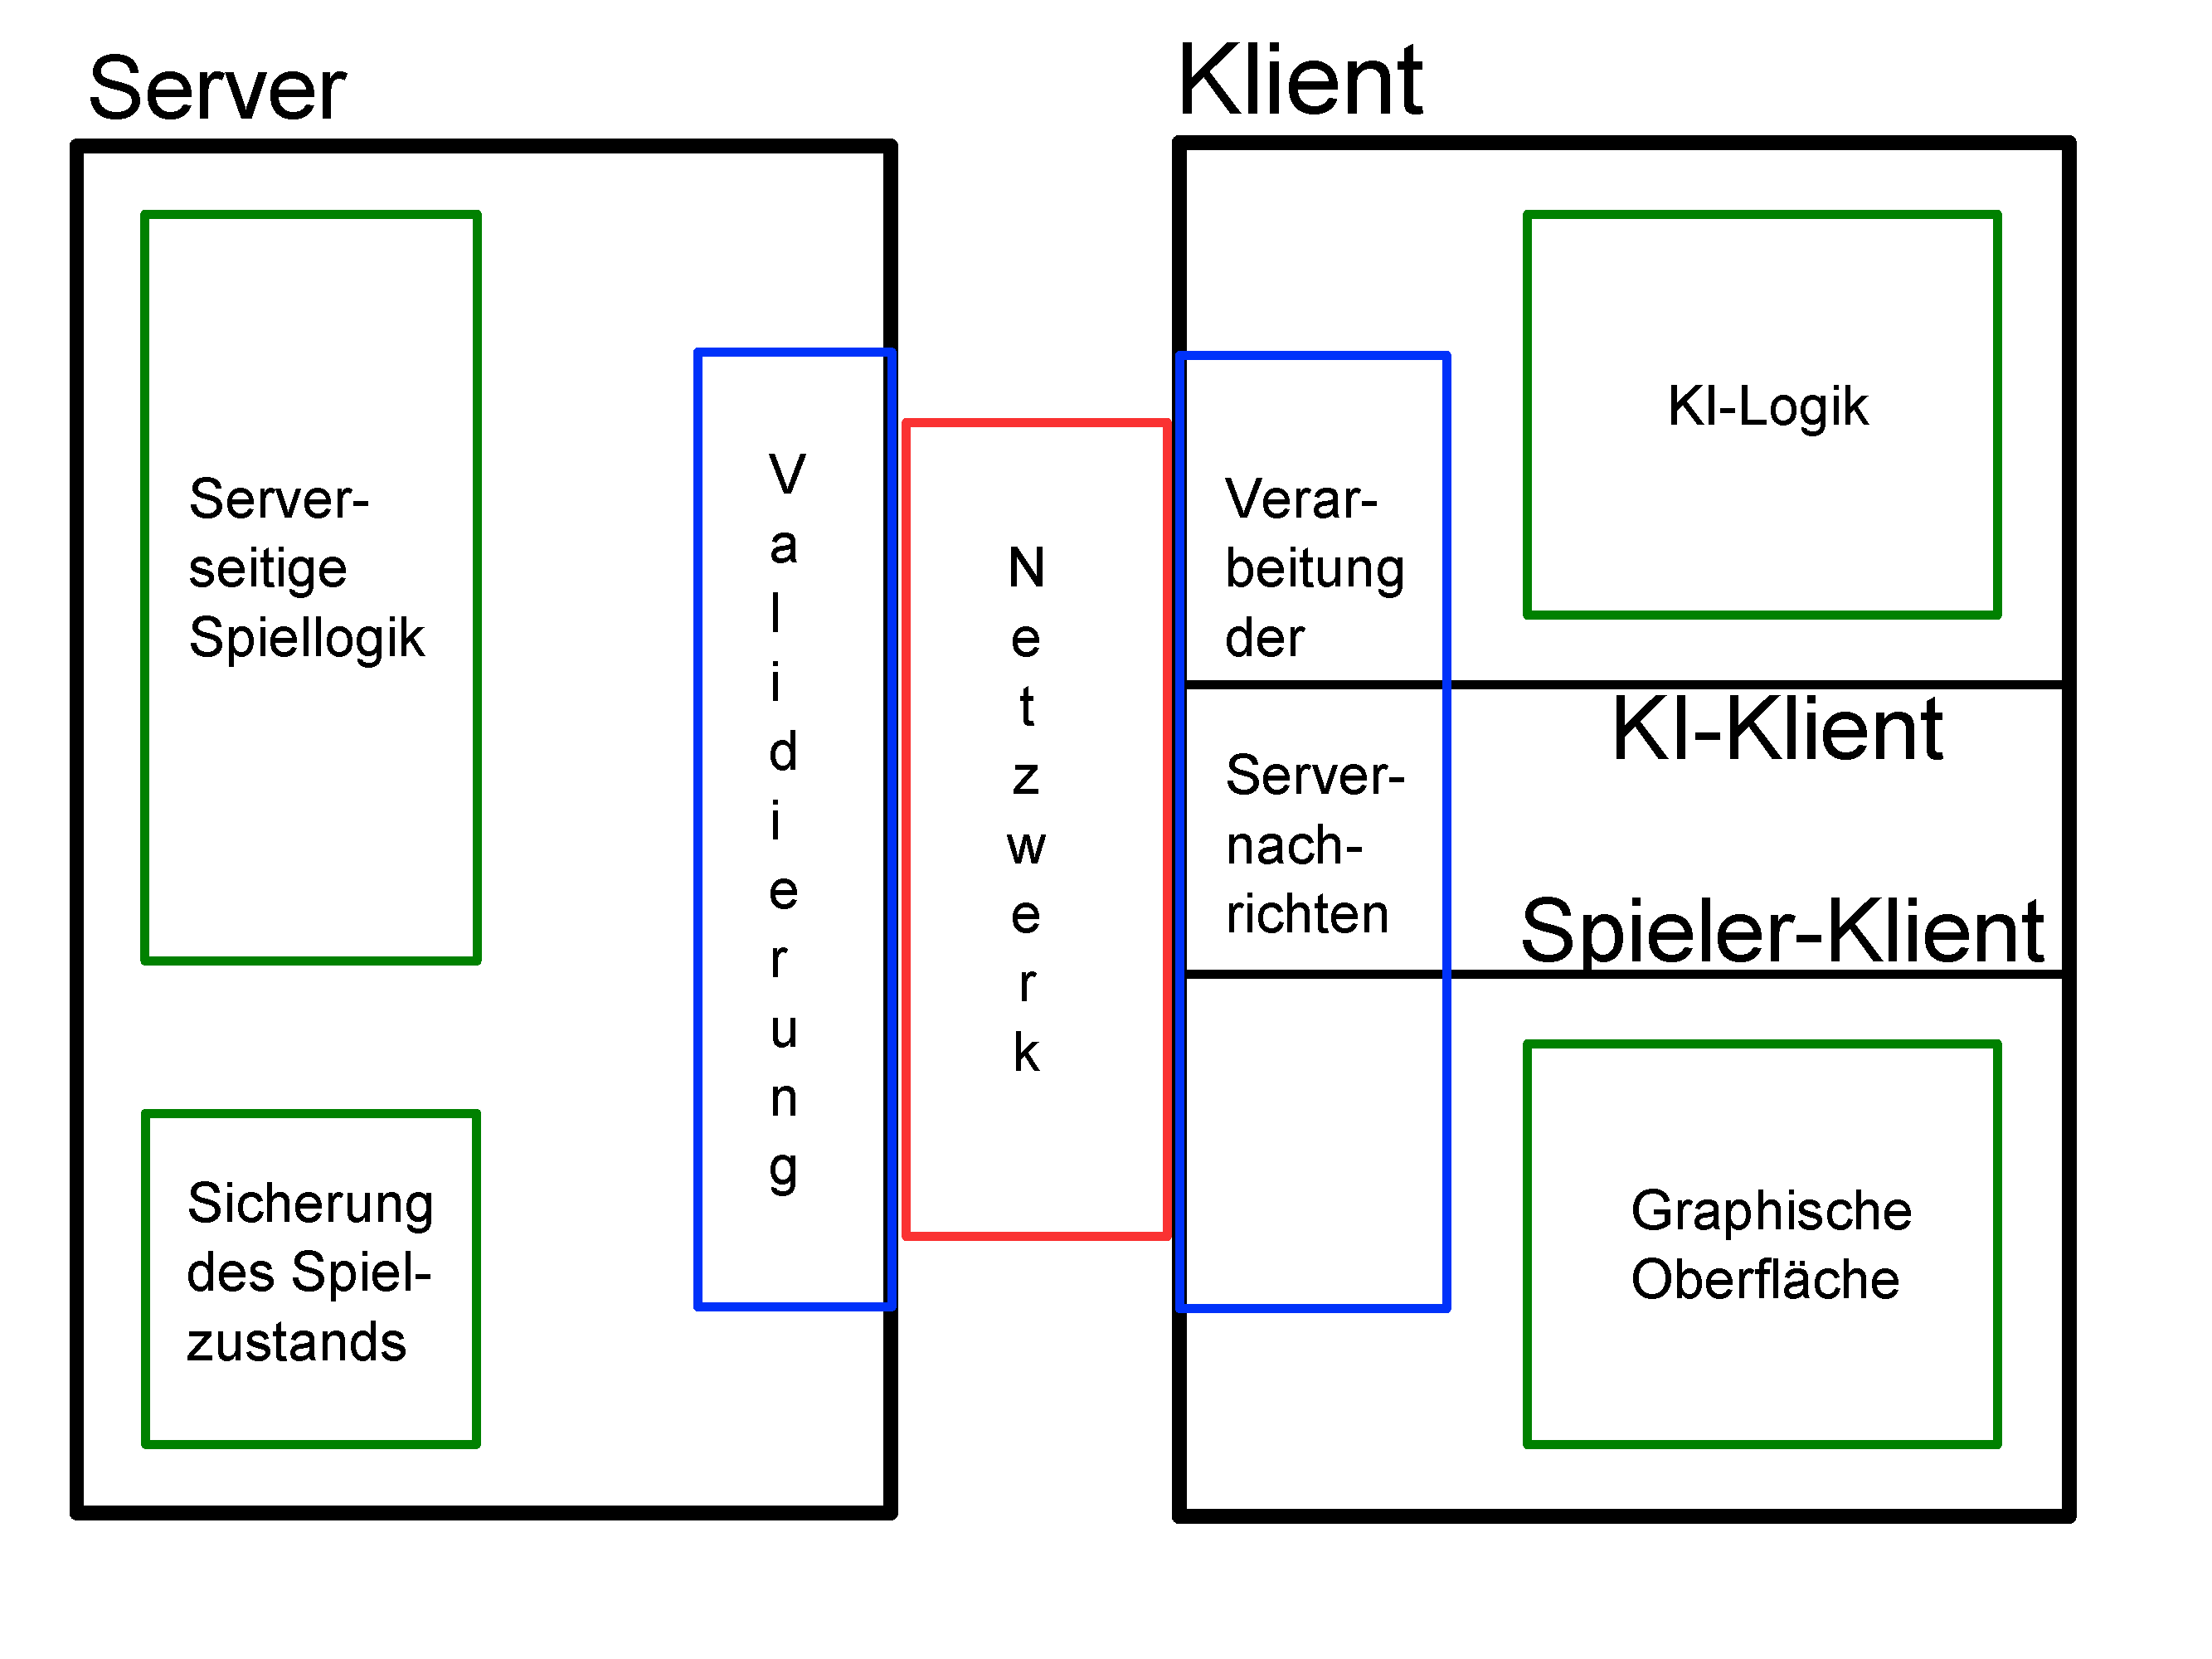
\includegraphics[height = 14cm]{systemmodell}

\section{Benutzungsoberfläche}
\subsection{Hauptmenü} 
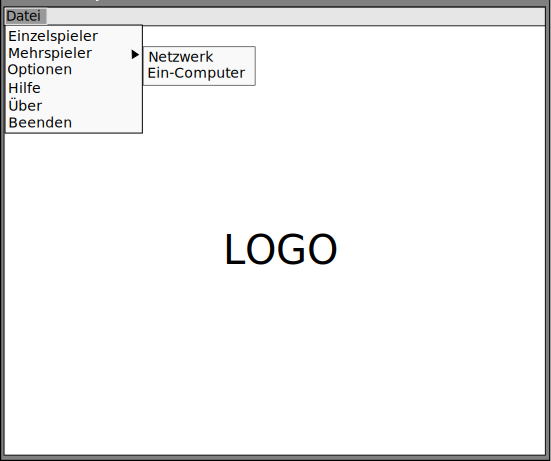
\includegraphics[height=14cm]{hauptmenue}  
\subsection{Warteraum}
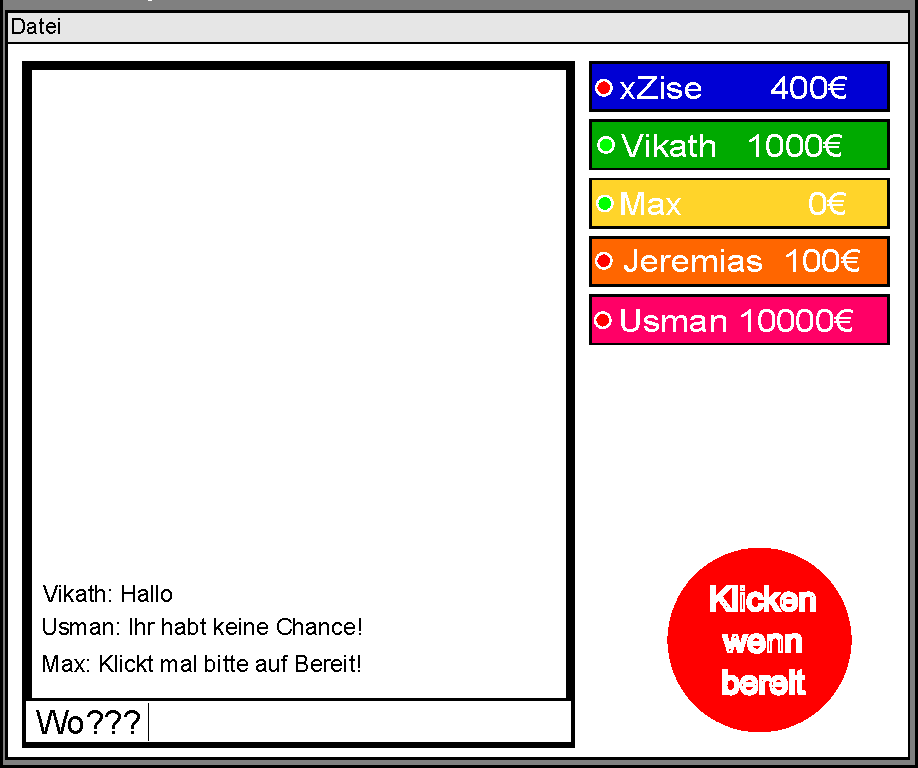
\includegraphics[height = 14cm]{warteraum}
\subsection{Spielfeld}
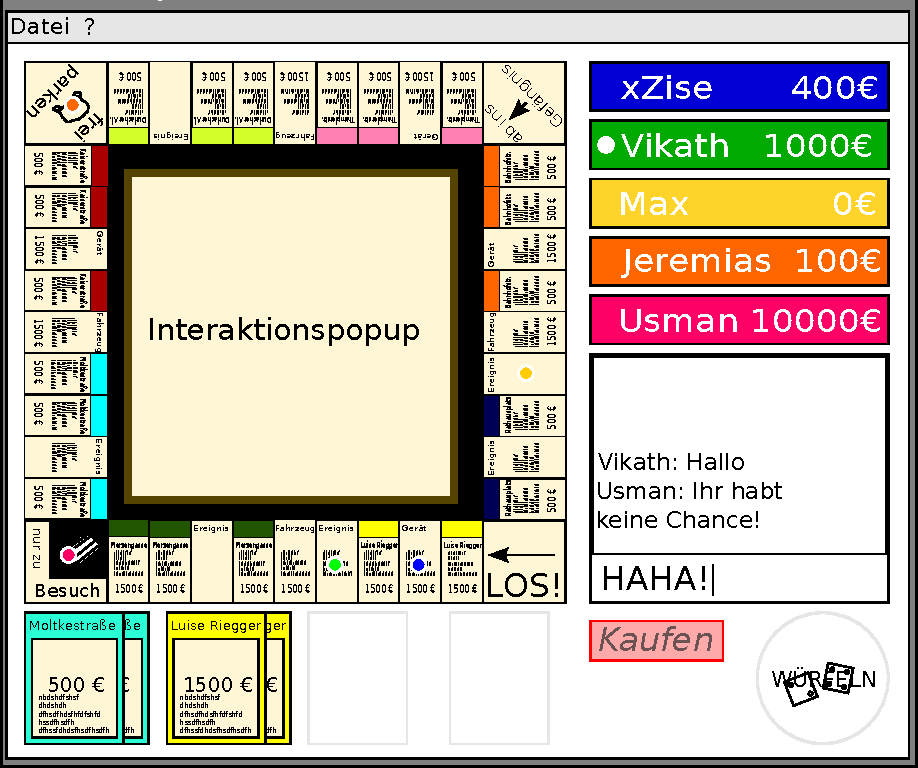
\includegraphics[height = 14cm]{spielfeld}

\section{Spezielle Anforderungen an die Entwicklungsumgebung}
\begin{itemize}
\item Allgemein
\begin{itemize}
\item \LaTeX
\item Versionskontrolle (SVN, Git)
\end{itemize}
\item Entwicklung
\begin{itemize}
\item IDE: Eclipse, Netbeans
\end{itemize}
\item  Entwurf
\begin{itemize}
\item Geeignete UML-Tools wie Rational Architect, DIA
\end{itemize}
\item Validierung
\begin{itemize}
\item JUnit
\end{itemize}
\item Teamkommunikation
\begin{itemize}
\item Forum
\item E-Mail (Verteiler)
\end{itemize}
\end{itemize}

\section{Zeit- und Ressourcenplanung}
\subsection{Projekt-Untergliederung}
\begin{tabular}[h]{l | r | l}
  \hline
  Zu planende und implementierende Module & Zeit & Personen\\
  \hline
  \hline
  KI-Spiellogik & 75h & Jeremias, Fabian \\
  Client-Grundgerüst & 40h & Fabian\\
  GUI - Design + Funktionalität & 30h & Philip, Max\\
  Menüführung + Funktionalität Klient & 20h & Usman\\
  serverseitige Spiellogik & 100h & Philip, Max\\
  Sicherung des Spielzustands & 20h & Usman\\
  Verifizieren der Klient-Eingabe & 10h & Jeremias\\
  Netzwerkanbindung & 20h & Usman\\
  \hline
\end{tabular} 

Präsentation des Pflichtenhefts: Philip Caroli
\subsection{Ressourcen}
\begin{itemize}
\item Rechner mit Leistungswerten in der Nähe der Mindestanforderungen
\item Zwei oder mehr über Netzwerk verbundene Rechner
\end{itemize}
\section{Glossar}
\begin{itemize}
\item Metaserver (syn. Masterserver) \\
Eine mögliche Ergänzung. Speichert die IPs von mehreren Servern, sodass sie in der Serverliste angezeigt werden können.
\item IDE Integrated Development Environment \\
Entwicklungstool, welches Editor, Compiler, Linker und Debugger enthält
\item Client \\
Ein Client ist ein Programm, welches zu einem Server Kontakt aufbaut und mit diesem Daten austauscht.
\item Server \\
Ein Server stellt Dienste für den Client bereit und tauscht Daten mit ihm aus.
\end{itemize}
\end{document}
